\section{Conclusion}
\subsection*{Mass Matrix Modeling}
Modeling the mass matrix of a robotic manipulator becomes increasingly difficult as the DOF of the system increase.
Our attempt to avoid this complexity was to model the mass matrix with a neural network.
To further decrease the dimensionality of the problem, it is well understood that the mass matrix is a positive definite (PD) square matrix.
Thus the neural network output only the lower triangle of the matrix, and the remaining values were copied from the output accordingly.
Once the mass matrix neural network was trained, it was used in simulation to develop a trajectory tracking controller.

%\subsection*{The Kalman Filter}
The Kalman Filter is used to mitigate the noise present in a system as the system moves.  The goal is to know what the robot is doing at the next time step, using the knowledge of the current time step.  The motion of the system is described by the following uncertainty model:
\begin{equation}
    x_{t=1}=Ax_t+Bu_t+v_t,
\end{equation}
where $v_t$ is a Gaussian noise variable pertaining to the uncertainty in the system behavior.
\\
The measurement made by the camera follows the uncertainty model
\begin{equation}
    y_t=Cx_t+w_t,
\end{equation}
where $w_t$ is a Gaussian noise variable describing the uncertainty in the camera's mapping of the environment.
\\
The Kalman Filter proceeds with a motion update that represents the motion of the model with noise:
\begin{equation}
    \mu_t^{pred}=A\mu_t+Bu_t
\end{equation}
\begin{equation}
    \Sigma_t^{pred}=A\Sigma_tA^T+R_v
\end{equation}
\\
After completing the motion, the camera makes a measurement update:
\begin{equation}
    K_t=\Sigma_t^{pred}C^{T}(C\Sigma_t^{pred}C^{T}+R_w)^{-1}
\end{equation}
\begin{equation}
    \mu_{t+1}=\mu_t^{pred}+K(y_t-C\mu_t^{pred})
\end{equation}
\begin{equation}
    \Sigma_{t+1}=(I-KC)\Sigma_t^{pred}
\end{equation}
\subsection*{Implementation}
Since the camera is attached to the end-effector, the measurements from the camera are made from the frame of the end-effector.  Since the system explores $\mathbb{R}^{3\times3}$, the Kalman Filter is created to handle three-dimensional space, ignoring orientations.  So, the robot $r$ and any landmark $L$ $\in\mathbb{R}^{3\times3}$.  The state is therefore a vector consisting of the robot and landmark x-y-z coordinates:
\begin{equation}
    x=\begin{bmatrix} x_r\\y_r\\z_r\\...\\L_{xi}\\L_{yi}\\L_{zi} \end{bmatrix}
\end{equation}
for i landmarks.
\\
Matrices A and B contain only non-zero elements on the main diagonal with entries of 1.  Matrix A has size $(3+3i)x(3+3i)$ and Matrix B is of size $(3+3i)x3$.  The matrix C describes the measurement as the distance between the landmark and the robot.  C is of size $(3i)x(3i+3)$.  The non-zero entries lie on the diagonals, with -1 entered on the corresponding robot state and 1 entered on the corresponding landmark state.
\subsection*{Control Model}
In order to implement the adaptive control in the Julia programming language, we needed a way to account for the adaptation law. This implementation was not initially very straightforward, as the ``simulate!()" function places certain restrictions on the inputs to the control function that we choose. To alleviate this issue, we made the adaptive controller a mutable structure which contains the adaptation parameter as a member. This implementation allows us to continually update the parameter, without having to troubleshoot issues associated with other methods.\\

With this control fully implemented, we then move to the full simulation of the control in which we track the state error and end-effector trajectory.
\begin{figure}[H]
	\centering
	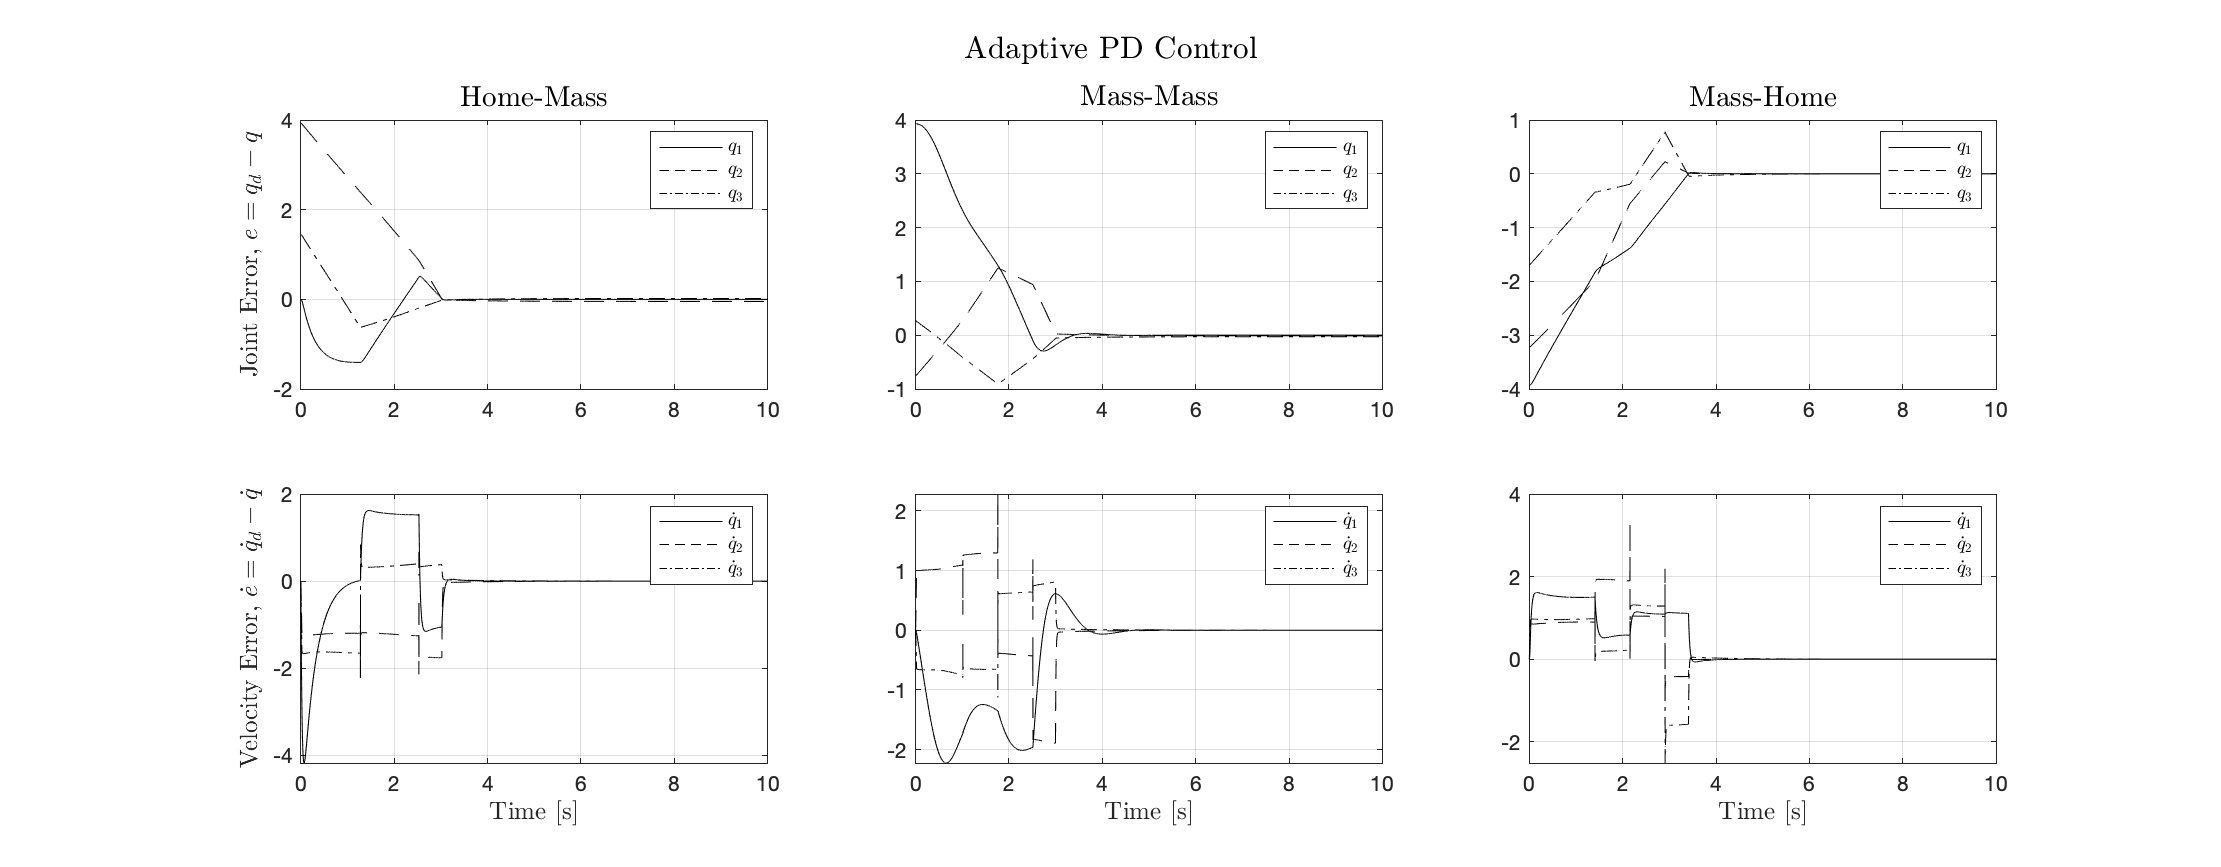
\includegraphics[width=\textwidth]{figures/mass10NNerrAPD.eps}
	\caption{Adaptive controller error in full simulation}
	\label{fig:nnerrapd}
\end{figure}
\begin{figure}[H]
	\centering
	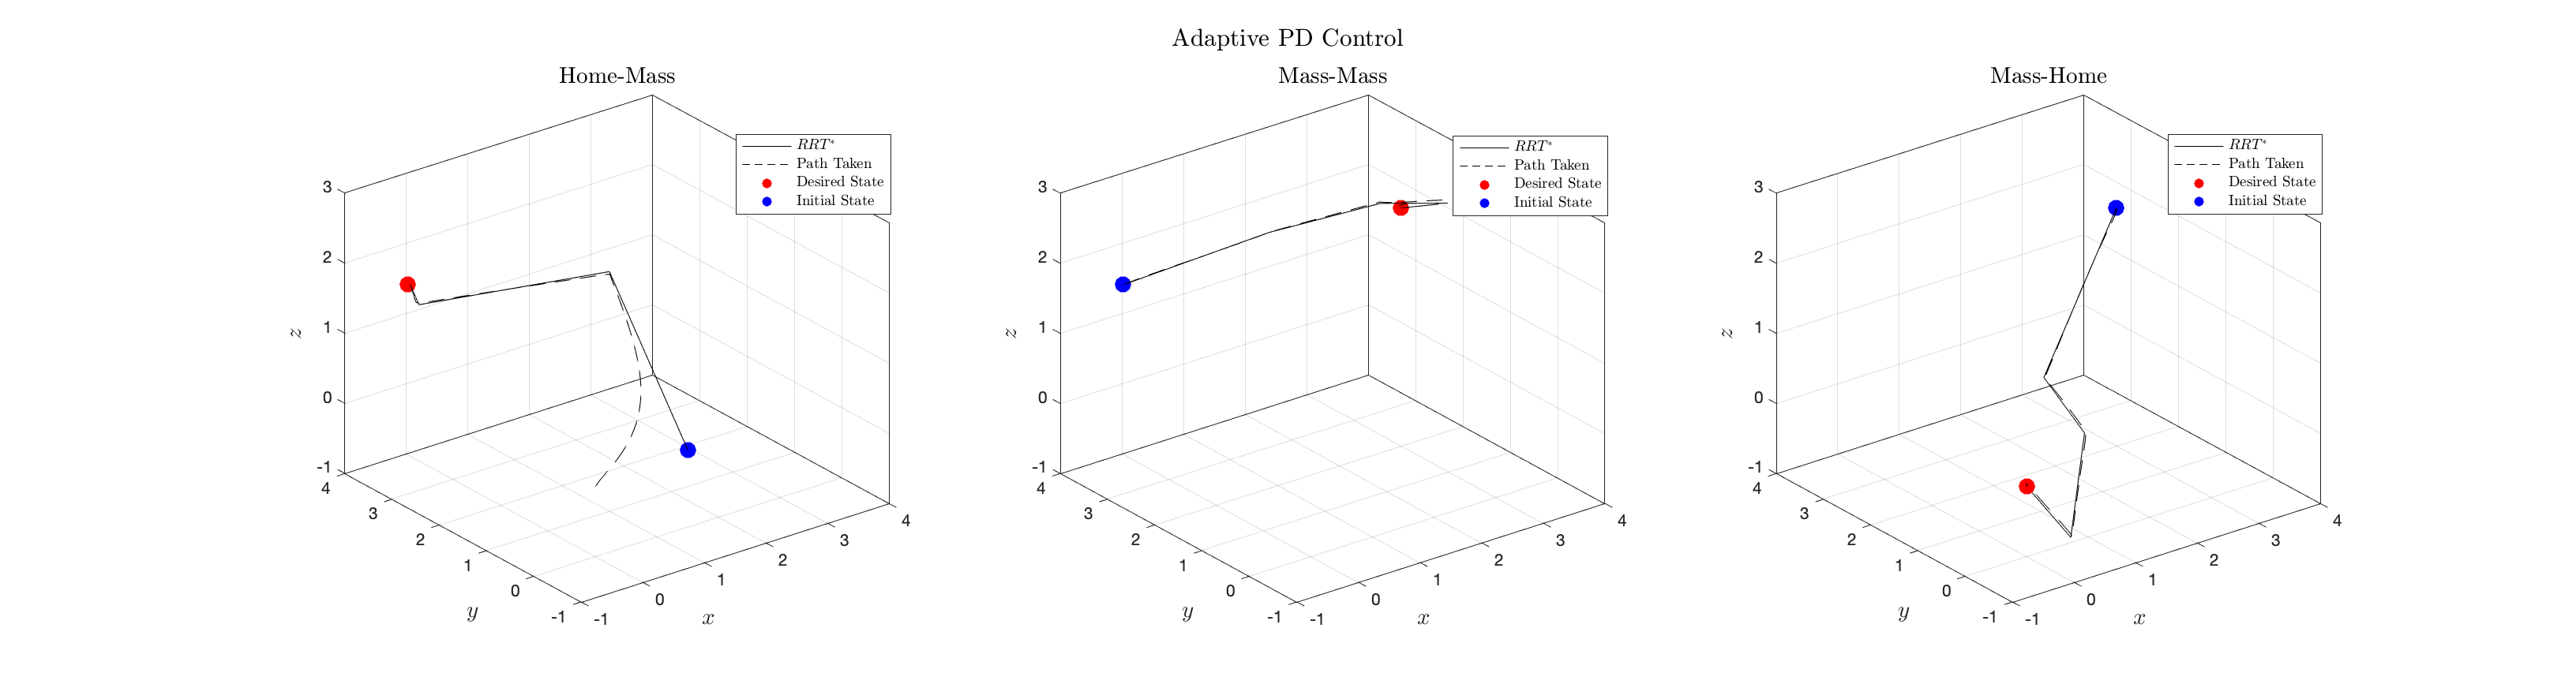
\includegraphics[width=\textwidth]{figures/mass10NNeetrajAPD.eps}
	\caption{End-effector trajectory with adaptive control}
	\label{fig:nntrajapd}
\end{figure}
\noindent We can see from Fig. \ref{fig:nntrajapd} that our initial error results in a false start position, however this error quickly decreases to zero as expected, and the trajectory is followed very tightly for the remainder of the simulation.

We then look at a mass estimated PD model, to observe the effects that an increase in mass has on the control.
\begin{figure}[H]
	\centering
	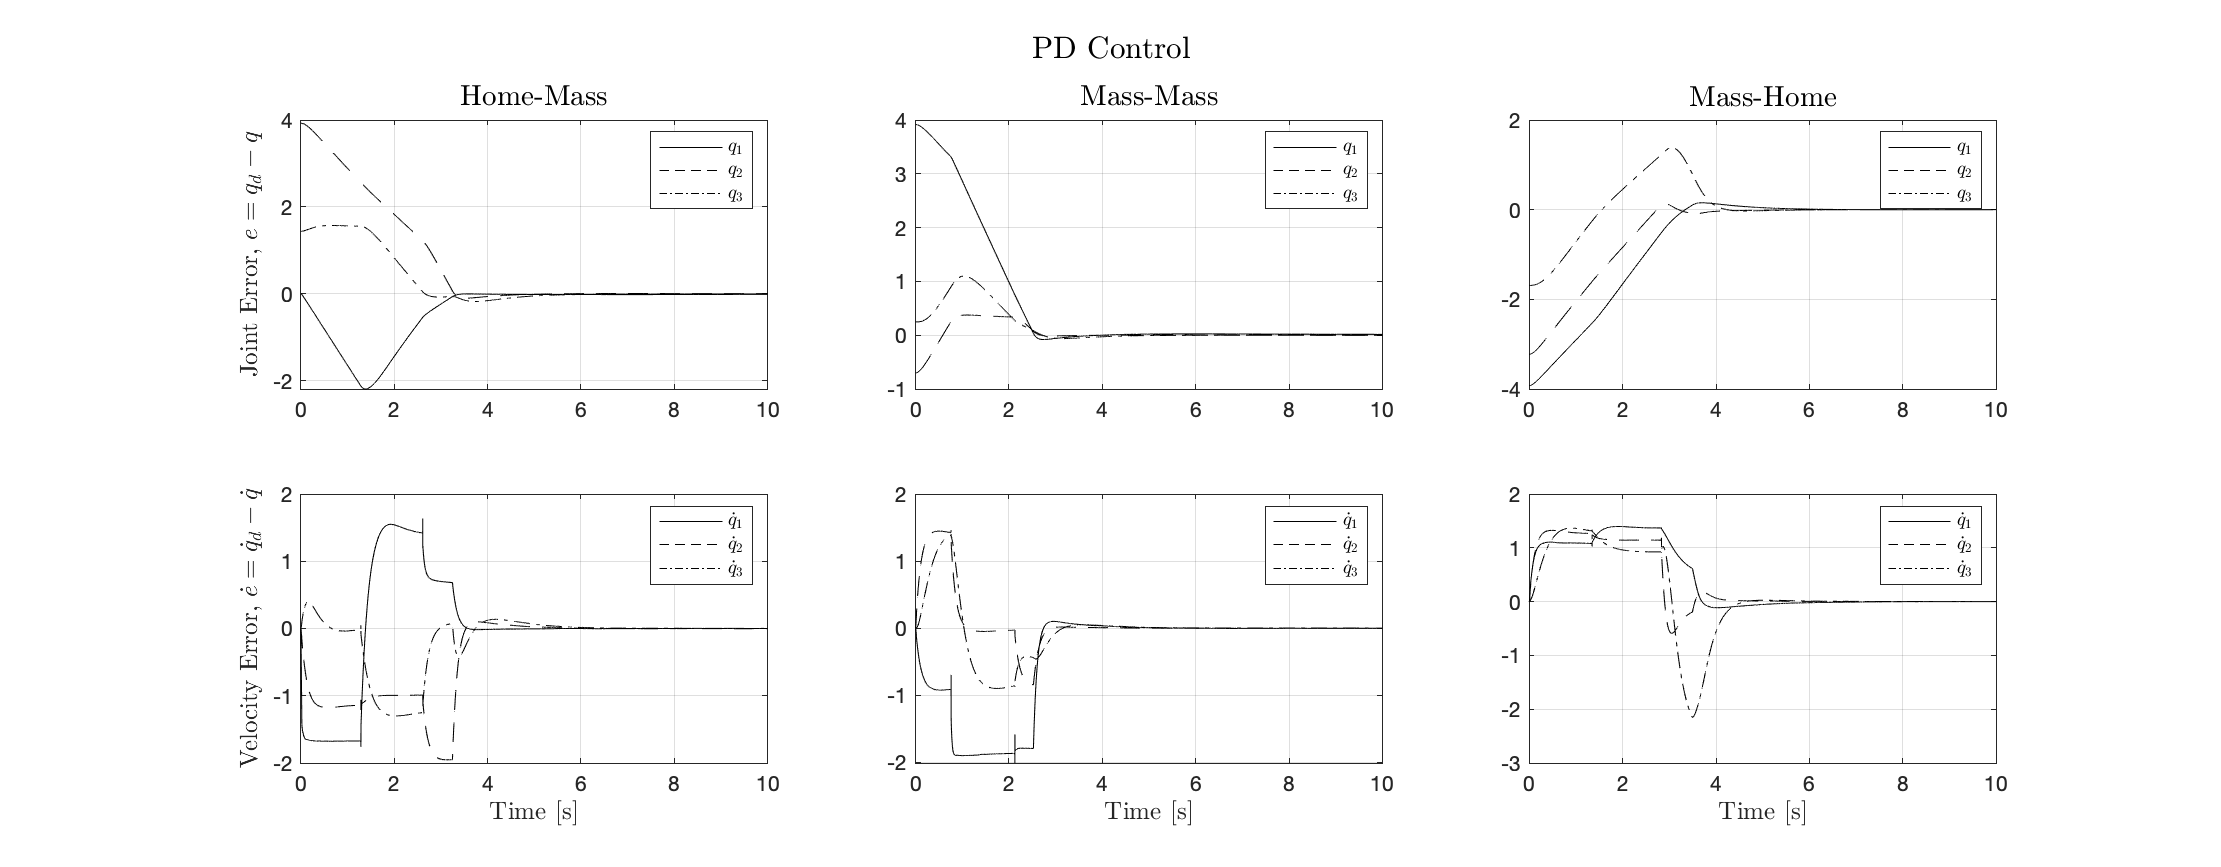
\includegraphics[width=\textwidth]{figures/mass10NNerrPD.eps}
	\caption{Mass estimated PD controller error in full simulation}
	\label{fig:nnerrpd}
\end{figure}
\begin{figure}[H]
	\centering
	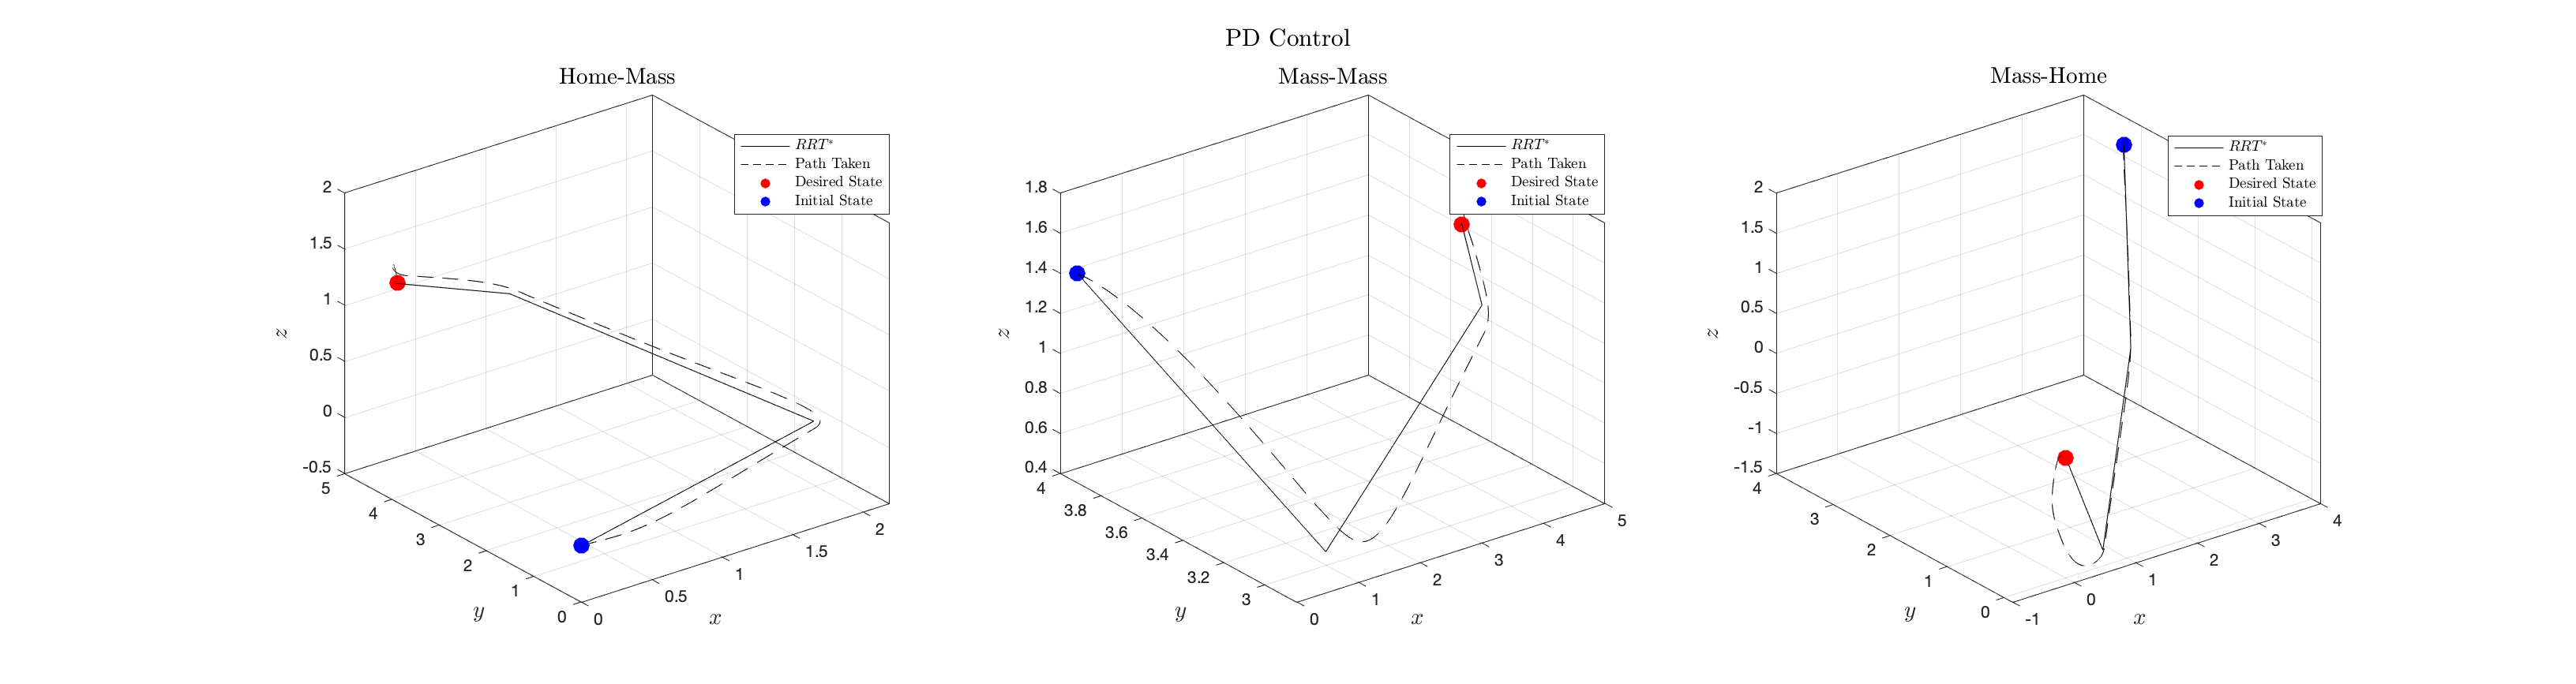
\includegraphics[width=\textwidth]{figures/mass10NNeetrajPD.eps}
	\caption{End-effector trajectory with mass estimated PD control}
	\label{fig:nntrajpd}
\end{figure}
\noindent In contrast to the adaptive model, the mass estimated PD controller places the end-effector in the desired start position.
However, we can easily see from Fig. \ref{fig:nntrajpd} that the PD control is not able to follow the desired trajectory as closely, and once the mass is picked up this issue worsens.


\subsection*{Challenges and Obstacles}
Many of the challenges and obstacles faced during this project related to the limitations within the Julia packages themselves for simulation.
The most difficult problem was the lack of control during the simulation of the dynamics themselves.
Since RigidBodyDynamics uses the ODESolver package, the dynamic steps are not controllable, and adaptive stepping is used when solving these ODEs.
On top of that, there is no easy and convenient method to pass state to and from the simulate function, meaning all state required, both as input and output, needed to be passed in as a functor before the function was called.
This lead to many bugs and debugging headaches.

Another limitation seemed to be in the way RigidBodyDynamics handled URDF file values.
In particular, it did not seem to honor any kind of static or dynamic friction models, meaning simulating with friction was not possible.

The visualization support was also very limited.
While MeshCat and MeshCatMechanisms boast several nice features for animations, we found these aspects of the packages to be unusable or difficult to figure out.
We ended up settling on some of the lower level animation functions, as their high level behavior and in-browser animation controls did not work for us.

One last issue was with the machine learning.
Flux, the de-facto package for machine learning in Julia appeared to have several broken aspects to it.
One in particular made it to where you could not train a model on a GPU if the input and output dimensions of the neural network did not match.
Since we were using a three DOF system, our mass matrix had input size 3 and output size 6, and there was a broadcasting Cuda error thrown when trying to run the model on the GPU.
It was still possible to run on the CPU, but trained much slower.

\subsection*{Lessons Learned}
The first lesson learned while implementing this project was the difficulty of working with high DOF systems.
While it should be obvious that increasing DOF will increase the complexity of nearly any non-trivial system, the degree by which it scales in robotics is brutal.
Thankfully we were able to limit the scope of our project to a three DOF system, which made implementing the code to our project much simpler.

Secondly, we got first hand experience in implementing several different types of controllers, including tracking controllers.
It was very rewarding to see our theory correctly applied to have the robot successfully navigate the obstacles in our world and follow the planned trajectories in simulation.
Our project combined many different facets of the material covered throughout the semester, so to see them all coordinating together was quite exciting.
